\chapter{Testování}
\label{6-testovani}

\section{IMU filtry}
Pro použítí ovládání drona byly uvažovány dvy filtry Mahonyho a komplementární. Jednotlivé filtry byly testovány, jak obrazově tak i numericky.\\
Obrazově byla testována reakce na pohyb a ustálení polohy.
Po reakční stránce a ustálení  polohy byl lepší komplementární filtr. Vzhledem k jednoduchosti filtru, reakční doba IMU jednotky je minimální. Výsledky jsou patrné z grafů.\\
Numericky byl testován rozptyl střední hodnoty. Byla použita data po ustálení polohy v časovém intervalu čtyř minut. Výsledky byly rovnocené, oba filtry měli rozptyl střední hodnoty v řádek setin stupně.\\
Pro ovládání drona je potřebná rychlá reakce IMU, proto byl použit komplementární filtr.\\
\begin{figure}[h]
	\centering
	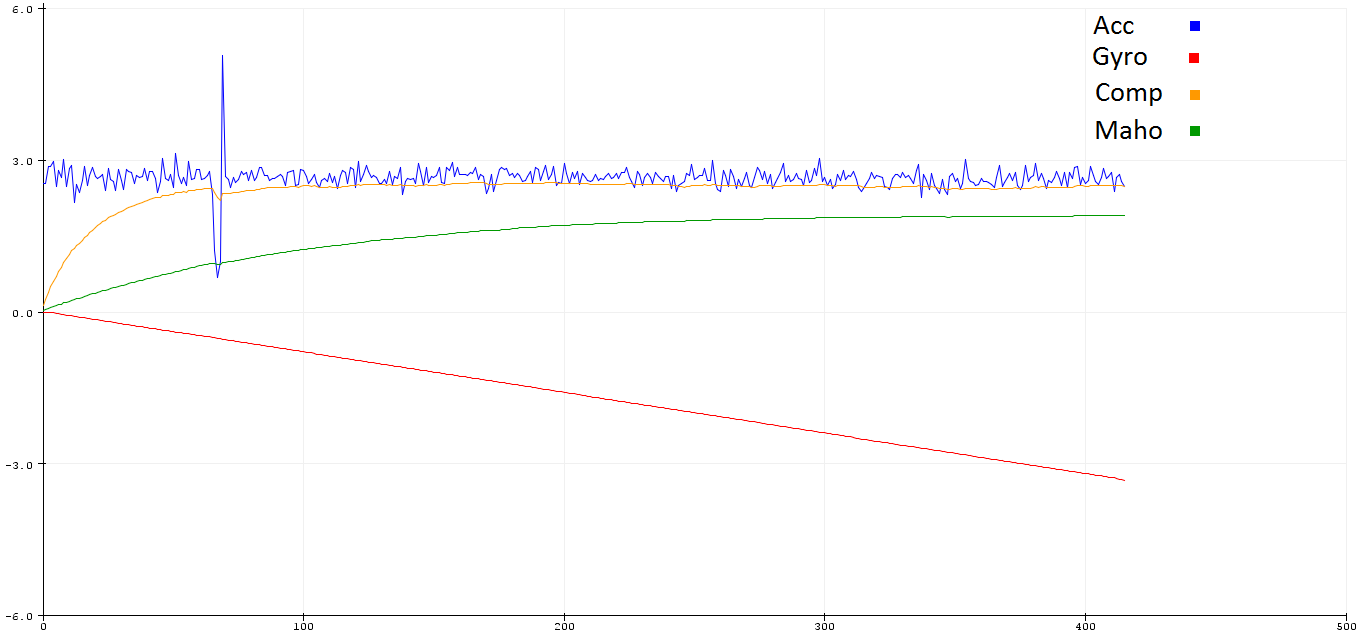
\includegraphics[width=14cm]{pictures/testRoll}
	\caption{Inicializace IMU}
\end{figure}

\begin{figure}[h]
	\centering
	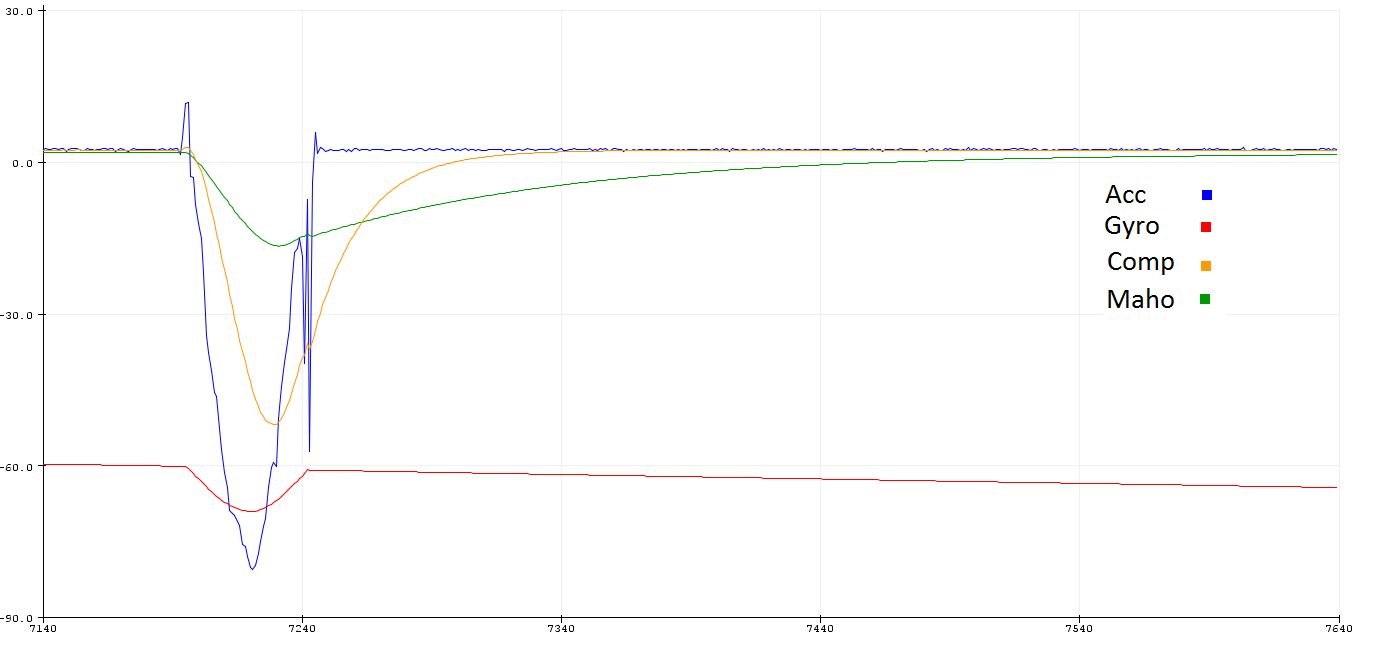
\includegraphics[width=14cm]{pictures/testRoll1}
	\caption{Náklon IMU jednotky}
\end{figure}

\section{Létající kontrolér}
Testování algoritmu létajícího kontorléru bylo prováněno na vyrobené konstrukci. Konstrukce se skládá ze čtyř latěk, které tvoří rám. Uprostřed je upevněná kovová trubka, na které se pohybuje dron. Dron je pevně připevněn k trubce tak, aby pohyboval po obvodu trubky. Na stranách trubky jsou umístěny molitanové pruhy kvůli tlumení nárazu stojánku drona. Konstukcí je docíleno simulování stavu letu s jedním stupněm volnosti. \\
Na konstrukci byla prováděna kalibrace PID regulátoru pro úhly pitch a roll. Kalibrace byla úspěšná při dostažení stabilizace drona na trubce. Kalibrace byla prováděna pro úhel pitch, výsledky kalibrace se použijí i pro úhel roll.\\
Prvně byl zjištován koeficient pro proporcionální složku. Koeficient bal navyšován do doby, než výkon vrtule dokázal drona srovnat z nakloněné polohy do vodorovné. Derivační koeficient byl zvyšován do doby, kdy PD regulátor dokázal drona stabilizovat ve vodorovné poloze. Integrační koeficient pouze doladil průběh PID regulátoru.\\


\begin{figure}[h]
	\centering
	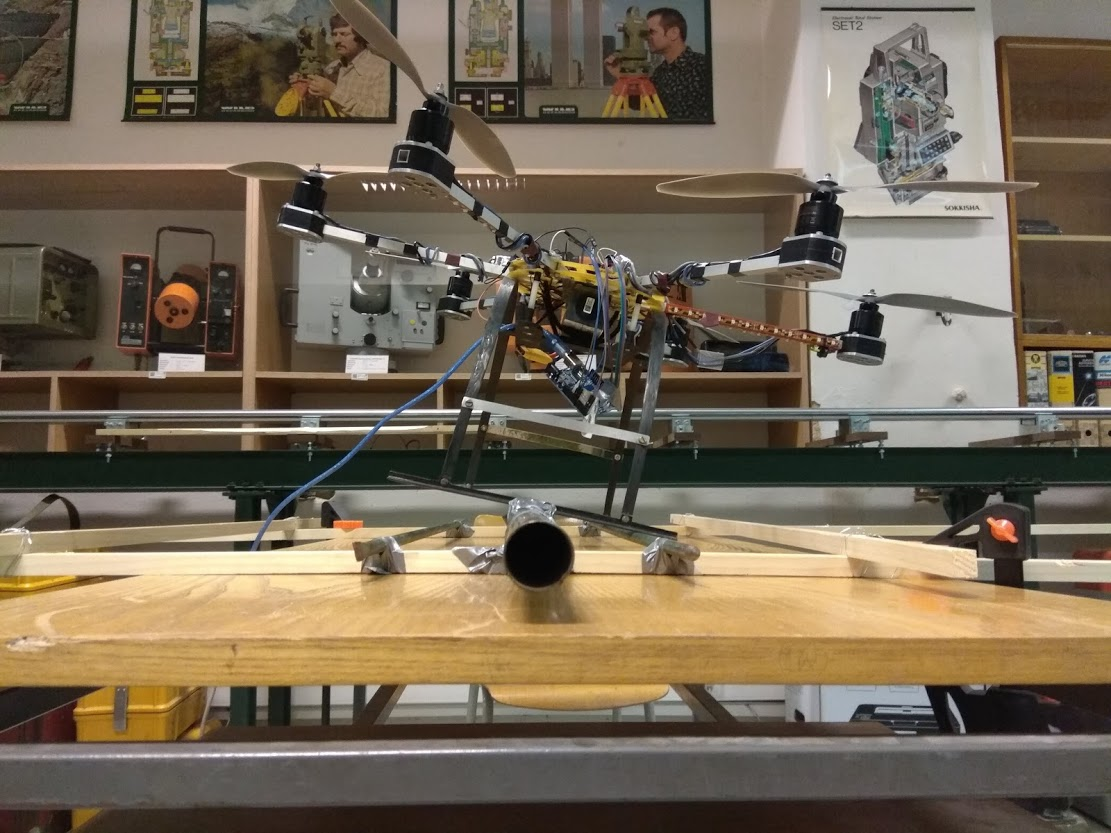
\includegraphics[width=10cm]{pictures/pidtest.jpg}
	\caption{Testování v konstrukci}
\end{figure}